\begin{center}
    \vspace*{1.5cm}
    {\fontsize{20}{20}\textbf{Punschvisor}}\\
    \vspace{0.7cm}
    {\fontsize{12}{12}\textit{Om sötsuget själv får välja}}
\end{center}
\addtocwithheader{Punschvisor}  % Add entry to TOC and set header\noBackground
\noBackground

\newpage
\resetBackground
  
  \subsection*{Punschen kommer (kall)} 
  \index[alfa]{Punschen kommer (kall)}
  \index[anfa]{Punschen kommer ljuv och sval}
  \songinfo{Mel: Vals ur Glada änkan}
  
  \begin{parse lines}[\noindent]{#1\\} 
    Punschen kommer, punschen kommer
    Ljuv och sval
    Glasen imma, röster stimma
    I vår sal
    Skål för glada minnen
    Skål för varje vår
    Inga sorger finnas mer
    När punsch vi får
  \end{parse lines}

  \subsection*{Punschen kommer (varm)} 
  \index[alfa]{Punschen kommer (varm)}
  \index[anfa]{Punschen kommer god och varm}
  \songinfo{Mel: Vals ur Glada änkan}
  
  \begin{parse lines}[\noindent]{#1\\} 
    Punschen kommer, punschen kommer
    God och varm
    Vettet svinner, droppen rinner
    Ner i tarm
    Skål för glada minnen
    Dem vi snart ej ha
    Då ett par glas simmig punsch
    Vi hunnit ta
  \end{parse lines}
    
  \newpage

  \subsection*{Djungelpunsch} 
  \index[alfa]{Djungelpunsch}
  \index[anfa]{Jag gillar alla tiders punsch}
  \songinfo{Mel: Var nöjd med allt som livet ger}
  
  \begin{parse lines}[\noindent]{#1\\}
    Jag gillar alla tiders punsch
    Punsch till frukost, punsch till lunch
    Punsch till förrätt, varmrätt och dessert
    Jag gillar punsch för vet du vad
    Rent kaffe gör ju ingen glad
    Nej, punsch för fulla muggar vill jag ha
    
    Med konjak du lockar
    Den bästa Renault
    Förlåt om jag chockar
    Och tar punsch ändå
    Och bjuder du någon förnäm likör 
    Så får du ursäkta, det kanske stör
    Men jag väljer hellre Grönstedts Blå
    En Cederlunds eller Flaggpunsch å
    Kanske har du ren Platin?
    
    Jag gillar punsch, så ge mig punsch
    Och jag är din
    (Ja, jag är din)
    För evigt din
    
  \end{parse lines}
    
  \newpage

  \subsection*{Punschens lov} 
  \index[alfa]{Punschens lov}
  \index[anfa]{Ja, punschen är och punschen var}
  \songinfo{Mel: Rövarevisan ur Folk och rövare i Kamomilla stad}
  
  \begin{parse lines}[\noindent]{#1\\} 
    Ja, punschen är och punschen var
    Och punschen skall förbliva
    En lidelse vi alla har
    Som ingen kan fördriva
    Ja, punschen tinar opp, såväl
    Som svalkar både kropp och själ
    Den botar begären och lindrar besvären
    Ja, punschen den gör både gott och väl
  \end{parse lines}

  \subsection*{När kaffet är serverat} 
  \index[alfa]{När kaffet är serverat}
  \index[anfa]{När kaffet är serverat}
  \songinfo{Mel: Mössens julafton\\
  Sångarstriden 1987}
  
  \begin{parse lines}[\noindent]{#1\\} 
    När kaffet är serverat och maten tagit slut
    Och alla dom som blivit alltför fulla kastats ut
    Då vill vi ha ett nytt glas med något gult och kallt
    Som höjer och förbättrar vår promillehalt
    
    Arrak, etanol och sackaros
    Med salt och vatten blir
    Den bästa blandning som kan fås
    Söt och smetig, rent utav viskös
    En sexton, sjutton glas så blir du medvetslös
    
  \end{parse lines}
  
  \vissteduatt{Visste du att E-sektionen genom åren och fram till 2017 haft flera \\
  personer anställda som Mackbarsprinsessa?}
  
  
  \newpage


  \begin{textblock*}{3cm}(2.6cm,8.2cm) % {width}(x, y)
    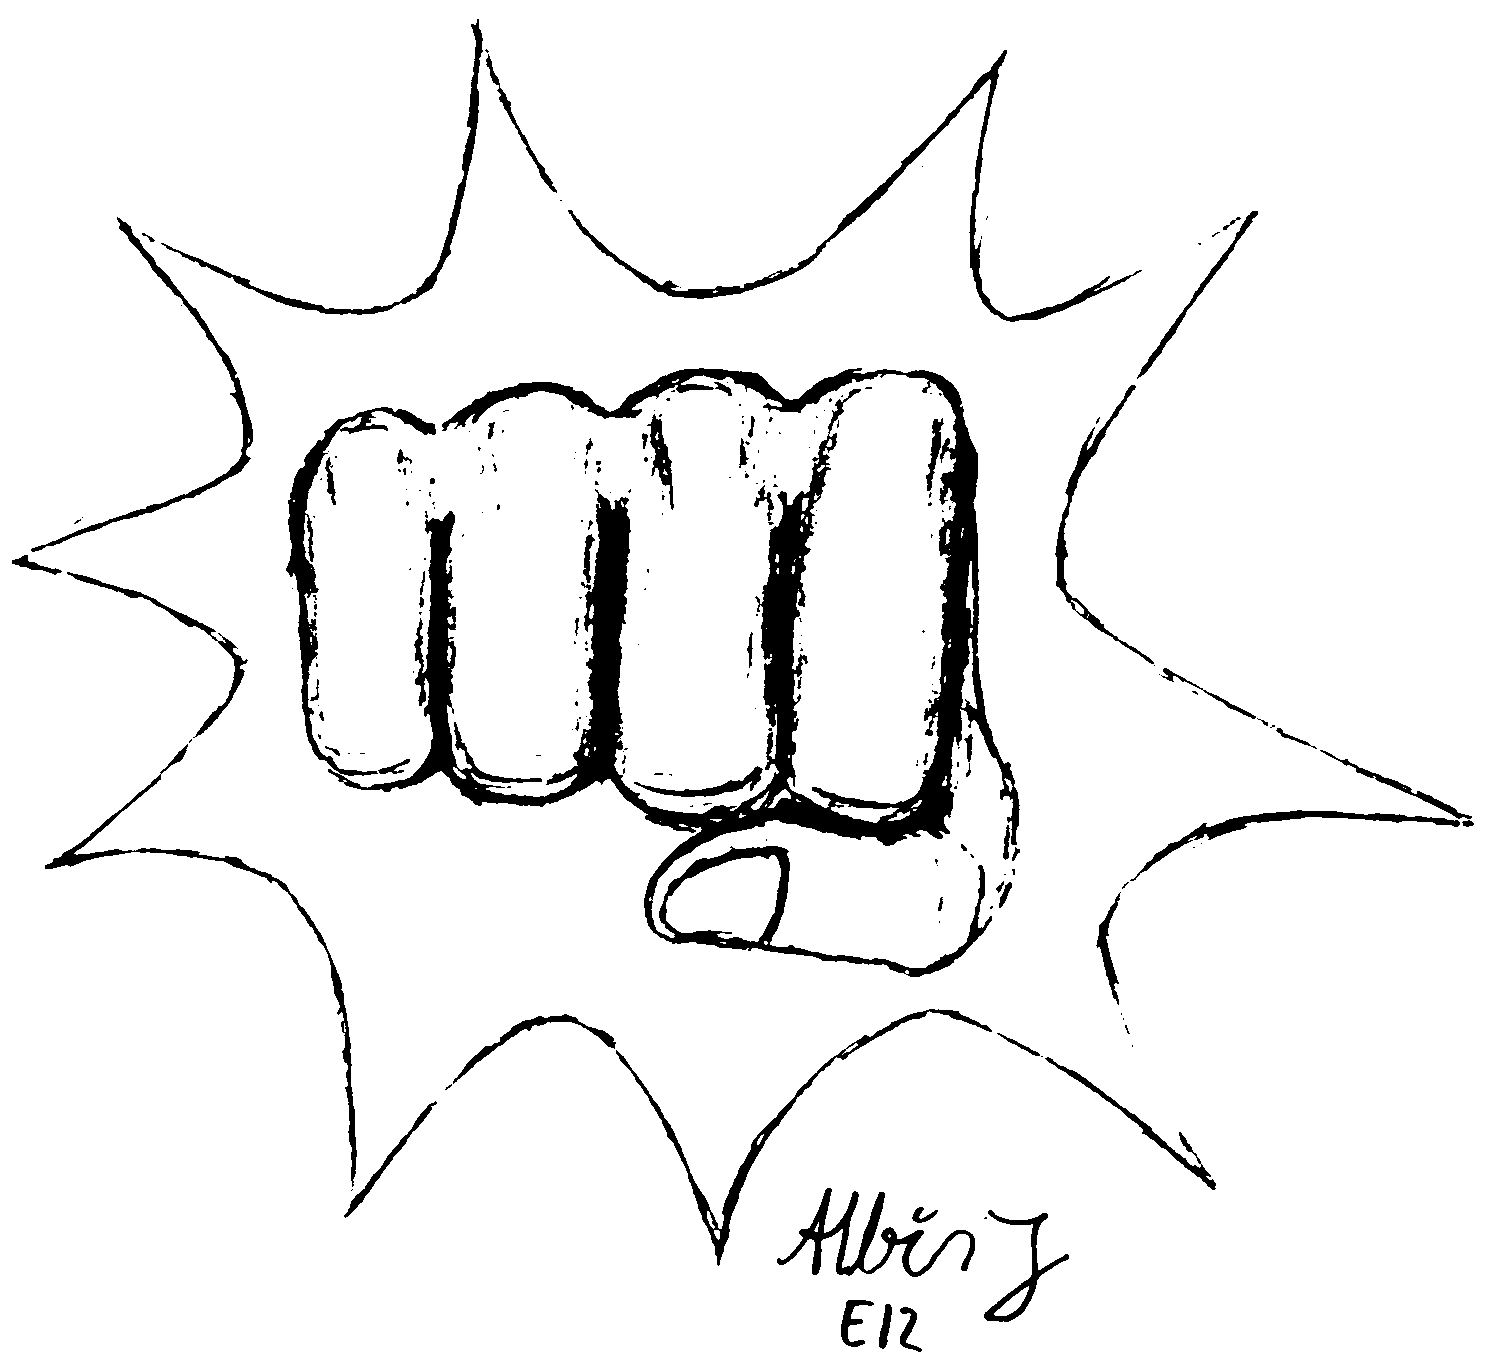
\includegraphics[width=6cm]{./bilder/punch.png}
  \end{textblock*}


  \subsection*{Punsch, punsch}
  \index[alfa]{Punsch, punsch}
  \index[anfa]{Punsch, punsch}
  \songinfo{Mel: Ritsch, ratsch}

  \begin{parse lines}[\noindent]{#1\\} 
    Punsch, punsch, fillibom-bom-bom,
    fillibom-bom-bom, fillibom-bom-bom
    Punsch, punsch, fillibom-bom-bom,
    fillibom-bom-bom, fillibom-bom-bom

    Vi har ju både Cederlunds och
    Carlshamns flagg, Grönstedts blå
    och lilla Caloric.

    Det blir för trist med 
    sodavatten, sodavatten, sodavatten
    Det blir för trist med sodavatten,
    nej, ge mig lite punsch!
  \end{parse lines}
\newpage

  \subsection*{Familjen Addams punsch} 
  \index[alfa]{Familjen Addams punsch}
  \index[anfa]{Vi vill ha punsch}
  \songinfo{}
  \begin{parse lines}[\noindent]{#1\\} 
    Vi vill ha punsch, \dag \dag
    Vi vill ha punsch, \dag \dag
    Vi vill ha punsch, vi vill ha punsch
    Vi vill ha punsch, \dag \dag
    
    När man vill festen liva
    Upp är det bra att kliva
    Omkring på bordets skiva
    Och klafsa runt i punsch
    
    Klafsa i punsch, \ddag \ddag
    Klafsa i punsch, \ddag \ddag
    Klafsa i punsch, klafsa i punsch
    Klafsa i punsch, \ddag \ddag
    
  \end{parse lines}
  \noindent\textit{
    \\
    \dag = knäpp med fingrarna\\
    \ddag  = sörpla med munnen 
  }
  \vissteduatt{Visste du att A-Sektionen 2014 hade nollningstemat Familjen Addams\\och att efter nollningen stod Phøsets gravstenar utanför IKDC?}
  
  \newpage
  
  
  \begin{textblock*}{3cm}(5.5cm,10cm) % {width}(x, y)
    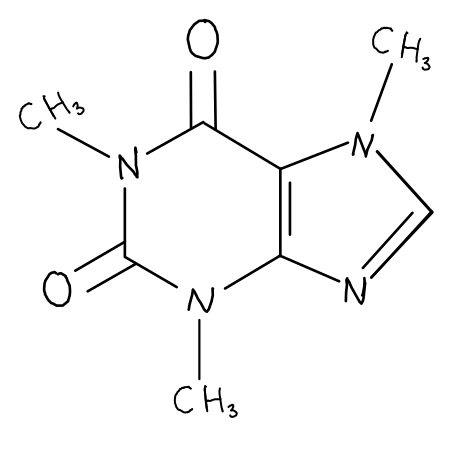
\includegraphics[width=4cm]{./bilder/majas-bilder/koffein.png}
  \end{textblock*}



  \subsection*{Kaffebönen} 
  \index[alfa]{Kaffebönen}
  \index[anfa]{Vi har ätit och vi mår så väldans bra}
  \songinfo{Mel: She'll be Coming 'Round the Mountain}
  
  \begin{parse lines}[\noindent]{#1\\} 
    Vi har ätit och vi mår så väldans bra
    Och nu vill nog säkert alla kaffe ha
    Snart så får ni höra stönen
    När vi sjunger kaffebönen
    Det skall höras ända bort till Stockholms sta'
    
    Kaffe, kaffe, kaffe, konjak och likör
    Ger åt alla här ett riktigt gott humör
    Och det kan ni ger er katten
    Vi ska sitta hela natten
    Dricka kaffe, kaffe, konjak och likör

    Ofta får man höra ordet kaffetant
    Husets herre säger gärna helt galant:
    “Du min rara, du min sköna,
    Älskar du din kaffeböna 
    Mer än mig, det kan väl inte vara sant?”
    
    Kaffe, kaffe, kaffe, konjak och likör…
    
  \end{parse lines}
  
  \newpage


  \subsection*{Punschen vi radat}
  \index[alfa]{Punschen vi radat}
  \index[anfa]{Punschen vi radat}
  \songinfo{Mel: Hemåt det bär \\ Sångarstriden 1978 } %\\ \colorbox{yellow}{V-sektionen, Sångarstriden 1978???}\\ Kursivt sjunges av sångförman}
  
  \noindent Punschen vi radat upp på vårt bord\\
  Ädlare dryck ej finns på vår jord\\
  Hur härligt härlig du står och väntar på mig\\
  Oh, vad jag älskar dig!\\

  \noindent\textit{Oh, ljuva punsch\\}
  Oh, ljuva punsch\\

  \noindent\textit{Uti, min hand\\}
  Uti, min hand\\

  \noindent\textit{Nu tar du plats\\}
  Nu tar du plats\\

  \noindent\textit{I magens famn\\}
  I magens famn\\

  \noindent\textit{Jag drack dig upp\\}
  Jag drack dig upp\\

  \noindent\textit{Och du rann ner\\}
  Och du rann ner\\
  
  \noindent Snart får du sällskap utav fler!
  
  \newpage